\chapter{Case Studies}
\section{Overview of Case Studies}
The case studies provide three distinct perspectives of applying Mobile Analytics to Android apps. Android apps were selected to enable the use of Google Play Console reports and analytics, including Android Vitals; nonetheless one of the case studies chose to also include analytics in their iOS app so this will also be covered briefly.

Early research explored ways developers of opensource Android apps use local logging, a complementary and oft used approach intended to help developers learn more about how their app behaves locally at run-time. 

\begin{table}[th]
    \centering
    \begin{tabular}{l|l|r|l}
      Case Study &Role of Researcher &Apps \\
      \hline
       \href{https://play.google.com/store/apps/dev?id=9116215767541857492&hl=en_GB}{Kiwix}  &Embedded &18 \\
       \href{https://play.google.com/store/apps/developer?id=Catrobat&hl=en_GB}{Catrobat} &Guide &6 \\
       \href{https://play.google.com/store/apps/developer?id=Moonpig.com&hl=en_GB}{Moonpig.com} &Observed &1 \\
       \href{https://play.google.com/store/apps/details?id=boundless.moodgym&hl=en_GB}{Moodspace app} &Interviewed &1 \\
       \href{https://play.google.com/store/apps/details?id=com.localhalo.app&hl=en_GB}{Local Halo app} &Observed &1 \\
    \end{tabular}
    \caption{Project teams and Commercial apps in the case studies}
    \label{tab:case_studies}
\end{table}

For the Kiwix case study, the researcher has been an intrinsic long-term member of the diffuse project team, able to work directly with the code-base and collaborate directly with the developers and ancillary members of the project team. 

For the Catrobat case study, the researcher advised and assisted the project team to apply mobile analytics to their larger, older, and less reliable app: \emph{Pocket Code}. The researcher helped lead a one-day hackathon and otherwise interacted through a bug reporting tool, JIRA, discussions and using shared documents. Pocket Code also included a crash-reporting library which allowed cross-tool comparisons of reports, analytics and data. During the research, the reporting platform for the crash-reporting was migrated to a newer service which provided further insights and comparisons across and between the various mobile analytics tools.

For the commercial app teams (Moonpig, Moodspace, and LocalHalo), the researcher corresponded with one of the development team for each of the commercial apps and received either direct access to their analytics tools (LocalHalo), or was provided with snapshots (Moonpig and Moodspace). Permission was granted by their respective organisations for their contributions to be used for research purposes.

\section{Kiwix Android Apps}
\subsection{Case study of working with the Kiwix team}
As reported in \cite{harty_google_play_console_insightful_development_using_android_vitals_and_pre_launch_reports} and \cite{harty_better_android_apps_using_android_vitals} the Kiwix Android app had a very high overall crash rate caused by several significant flaws in the app. The project team released version 2.5 of the main Kiwix app in July 2019. As figure \ref{fig:kiwix_crash_rate_drops_v2_5} shows, the crash rate decreased significantly as version 2.5. In the last 30 days the crash rate was 1.87\% down from 5.07\% in February 2019.

One of the major changes in version 2.5 was the replacement of the in-house download utility with the default Android Download Manager\cite{kiwix_release_2_5_0}. The in-house version was a major source of crashes, and the replacement obviated a class of crashes, however it did so at a price in terms of functionality and usability. The in-house download utility allowed users to pause and resume downloads, and it would complete failed partial downloads. Users also received updates on the progress of the downloads, important when they often took many minutes or even hours or days in some cases (such as for multi-GB downloads over poor, slow, unreliable connections on low-end devices).
\begin{figure}
    \centering
    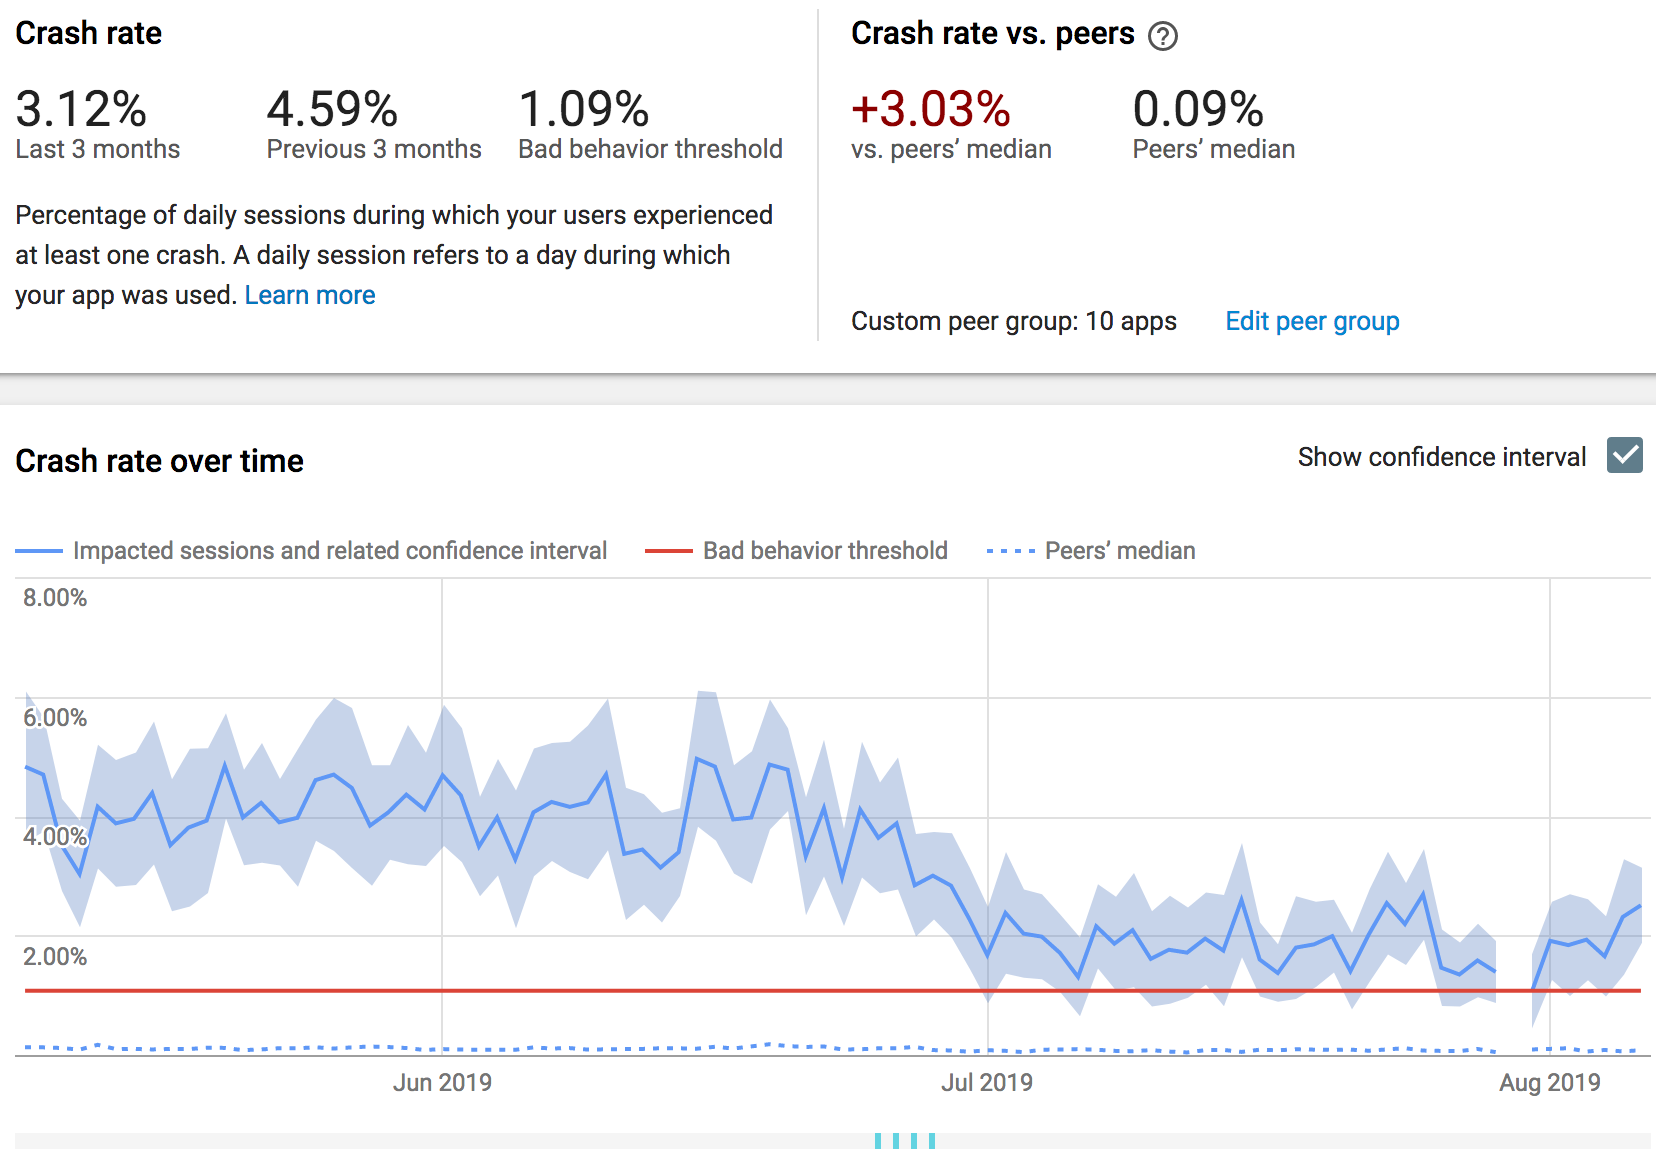
\includegraphics[width=\textwidth]{images/android-vitals-screenshots/kiwix-crash-rate-drops-with-v2_5.png}
    \caption{Kiwix Crash Rate Drops with V2.5 Release}
    \label{fig:kiwix_crash_rate_drops_v2_5}
\end{figure}

Following initial discussions about the crashes being reported in Android Vitals for version 2.5.0 of the Kiwix application, we collaborated on a week-long hackathon in Stockholm in August 2019. There, the developers ended up fixing some of the causes of the most frequent crashes with a surprisingly small amount of code of under 25 lines (including 10 lines of text added to the release log)\footnote{\url{https://github.com/kiwix/kiwix-android/pull/1388}}.

Several developers for the Kiwix project, the lead developer in particular, have been actively reviewing crashes reported by Android Vitals, filing issues, and addressing the causes of the crashes in order to reduce the crash rate and improve the app's stability. Evidence issues that mention crash: 133 closed, 6 open. \footnote{\url{https://github.com/kiwix/kiwix-android/issues?utf8=\%E2\%9C\%93&q=is\%3Aissue+crash}}
%TODO in a longer work, analyse each issue to identify the source of the crash.

Several releases later, each with various changes and improvements aimed at fixing causes of crashes the crash rate was materially lower than when we started, at the time of writing the overall crash rate for the last 7 days is 0.54\% which is inflated because the rash rate for the previous release (3.1.2) spiked at 1.38\%, compared to 0.18\% for release (3.0.5 -  the last production release) and 0.25\% for the recently released fix (3.1.3).


\section{Catrobat Android Apps}
TBC

\subsubsection{Catrobat iOS App}
TBC
\section{Field Reports from Commercial App Developers}
TBC

\section{Research in logging practices}

\begin{itemize}
    \item Our research.
    \item The opensource tools we created to facilitate the testing and analysis of logging by Android developers.
    \item Explorations in methods to improve the effectiveness of logging and the analysis of log messages generated by apps.
\end{itemize}




\section{Summary of Case Studies}
The case studies includes a useful range of Android apps developed by independent teams using a variety of programming languages, mindsets, objectives, and constraints. In each team they learned to actively focus on stability metrics as reported in various technology-facing analytics tools, and the developers continue to see the merit of doing so on an ongoing basis.